\documentclass[letterpaper]{scrartcl}
\usepackage{lmodern}
\usepackage{amssymb,amsmath}
\usepackage{ifxetex,ifluatex}
\usepackage{fixltx2e} % provides \textsubscript
\ifnum 0\ifxetex 1\fi\ifluatex 1\fi=0 % if pdftex
  \usepackage[T1]{fontenc}
  \usepackage[utf8]{inputenc}
\else % if luatex or xelatex
  \ifxetex
    \usepackage{mathspec}
    \usepackage{xltxtra,xunicode}
  \else
    \usepackage{fontspec}
  \fi
  \defaultfontfeatures{Mapping=tex-text,Scale=MatchLowercase}
  \newcommand{\euro}{€}
\fi
% use upquote if available, for straight quotes in verbatim environments
\IfFileExists{upquote.sty}{\usepackage{upquote}}{}
% use microtype if available
\IfFileExists{microtype.sty}{%
\usepackage{microtype}
\UseMicrotypeSet[protrusion]{basicmath} % disable protrusion for tt fonts
}{}
\usepackage[margin=1in]{geometry}
\usepackage{graphicx}
\makeatletter
\def\maxwidth{\ifdim\Gin@nat@width>\linewidth\linewidth\else\Gin@nat@width\fi}
\def\maxheight{\ifdim\Gin@nat@height>\textheight\textheight\else\Gin@nat@height\fi}
\makeatother
% Scale images if necessary, so that they will not overflow the page
% margins by default, and it is still possible to overwrite the defaults
% using explicit options in \includegraphics[width, height, ...]{}
\setkeys{Gin}{width=\maxwidth,height=\maxheight,keepaspectratio}
\ifxetex
  \usepackage[setpagesize=false, % page size defined by xetex
              unicode=false, % unicode breaks when used with xetex
              xetex]{hyperref}
\else
  \usepackage[unicode=true]{hyperref}
\fi
\hypersetup{breaklinks=true,
            bookmarks=true,
            pdfauthor={Gus Dunn},
            pdftitle={Gloria-Soria (ddRAD58)},
            colorlinks=true,
            citecolor=blue,
            urlcolor=blue,
            linkcolor=magenta,
            pdfborder={0 0 0}}
\urlstyle{same}  % don't use monospace font for urls
\setlength{\parindent}{0pt}
\setlength{\parskip}{6pt plus 2pt minus 1pt}
\setlength{\emergencystretch}{3em}  % prevent overfull lines
\setcounter{secnumdepth}{5}

\title{Gloria-Soria (ddRAD58)}
\author{Gus Dunn}
\date{2014-12-29}
\usepackage{fontspec}
\setmainfont{Linux Libertine O}

% blockquote


\begin{document}
\maketitle

{
\hypersetup{linkcolor=black}
\setcounter{tocdepth}{3}
\tableofcontents
}
\section{Linkage disequilibrium}\label{linkage-disequilibrium}

The mean bin-wise LD decays with physical distance to 0.2 (half of
maximum value) near 708 bp and to the value of the 95th percentile value
(r\^{}2 = 0.12) near 10,570 bp of SNP-pair separation (Figure
\texttt{ld\_decay\_by\_physical\_distance}). We identified SNP-pairs
with outlier LD values within specific separation-bins using a custom
MAP-based filter. From a total of 6,454,294 SNP-pairs considered, 24,372
(0.38\%) were assigned corrected p-values \textless{}= 0.01. These
filtered SNP-pairs were compared against top SNPs from the selection
analyses (supplemental table
\texttt{ld\_filtered\_snps\_interest\_JOINED\_ANNOS\_grouped.xls}).

One hundred twenty five genes (52 with functional annotations) were
identified within 1000 bp of at least one SNP identified in
\texttt{Top10\_InfectionOverall} (41 genes, 18 with annotations for
\texttt{Top05\_InfectionOverall}). Among the most frequently occurring
annotations for these genes in the biological process (BP) domain were
transmembrane transport; transcription, DNA-templated; ion transport;
and metabolic process. In the molecular function (MF) domain, some of
the most frequently occurring terms were zinc ion binding; DNA binding;
transferase activity; and oxidoreductase activity.
\texttt{Selected\_PopPairwiseMSNB\_Environm} had no overlap with the LD
filtered SNP-pairs. \texttt{Top10\_PopPairwiseOverlap\_Infection} and
\texttt{Top10\_PopPairwiseOverlap\_Environm} both contained only the
same two SNPs in common with the LD filtered set. This SNP-pair (r\^{}2
= 0.9456, adjusted p-value = 0.0017, genomic coordinates =
Scaffold150:138,509;404,077) is separated by 265,568 bp, and each SNP is
located near annotated genes. Scaffold150:138,509 is within GFUI009292,
an ortholog of huckebein; Scaffold150:404,077 is 718 bp from GFUI009351,
a predicted gene with no recognized protein domains but an ortholog
predicted in \emph{Glossina palpalis}. Sixteen genes were located within
1000 bp of at least one of the 19 SNPs in
\texttt{Selected\_PopPairwiseMSOT\_Environm} that were also in the LD
filtered set. Six of these had functional annotations assigned by Argot2
including small GTPase mediated signal transduction, glycogen
biosynthetic process, carbohydrate metabolic process, and dorsal/ventral
axis specification in the BP domain and nucleotide binding, hydrolase
activity, transferase activity, and helicase activity in the MF domain.

\begin{figure}[htbp]
\centering
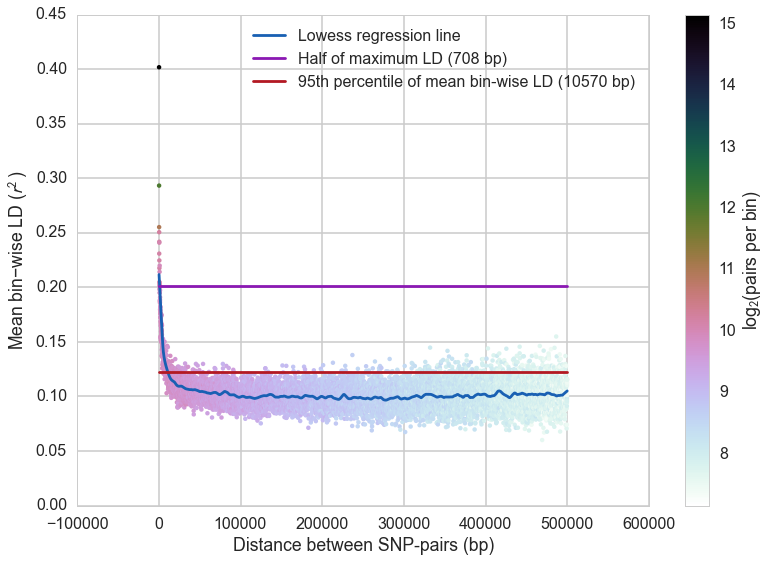
\includegraphics{../figures/ld_decay_by_physical_distance.png}
\caption{\textbf{Linkage disequilibrium decay with physical distance}.
Each ``dot'' represents the mean LD for that set of binned SNP-pairs.
The color of the dot illustrates the number of SNP-pairs contributing to
the mean. The blue colored line is a lowess regression line of best fit.
The purple colored line marks the LD value of one half the maximum while
the brick colored line is the LD value at which 95\% of the bins have
mean LD values below this value.}
\end{figure}

\end{document}
